\documentclass{article}
\usepackage[utf8]{inputenc}


\usepackage[margin=1in,top=1in,bottom=1in]{geometry}
\usepackage[pdftex]{graphicx}
\usepackage{tikz}
\usetikzlibrary{shapes,arrows,patterns,decorations.pathreplacing, decorations.markings,positioning,calc,decorations.pathmorphing}
\usepackage{setspace}
\usepackage{epstopdf}
\usepackage{caption}
\usepackage{enumitem}
\usepackage{pdfpages}
\usepackage{placeins}
\usepackage{subcaption}
\usepackage{amsmath}
\usepackage{empheq}
\usepackage{cancel}
\usepackage{xcolor}
\usepackage{etoolbox}
\usepackage{soul}
\usepackage{listings}
\lstset{
       basicstyle=\footnotesize\ttfamily,
       backgroundcolor=\color{lightGray},
       frame=single,
%        basicstyle=\footnotesize\sf,
       captionpos=b,
       tabsize=2,
       keepspaces=true,
       breaklines=true,
       postbreak=\mbox{\textcolor{red}{$\hookrightarrow$}\space},
  }
\usepackage{color}
\definecolor{lightGray}{rgb}{0.95,0.95,0.95}

% The call to include hyperref must be after most of the other packages are called.
% One notable exception it that hyperref must come before cleveref.
% Basically keep these two packages at the end of the \usepackage{} calls, in this order.
\usepackage[pdftex,
            hidelinks,
            pdfauthor={Evan Brunton},
            pdftitle={MAE 3302 --- Project Part 1},
            pdfsubject={Thermodynamics 2}
            ]{hyperref}


\usepackage[capitalize]{cleveref}
\newcommand{\creflastconjunction}{,~and~} % page 12 of the manual to get serial comma correct

\graphicspath{{Figures/}}

\title{Conceptual Design of a Combined Gas Turbine and Steam Turbine Power Plant}

\date{\today}

\author{Evan B, Brunton\\[2ex]
    UCCS Department of Mechanical\\
    and Aerospace Engineering
}

\begin{document}

\maketitle

\section{Introduction}

    This study will analyze a conceptual combined gas and steam turbine power plant. Initially, atmospheric air is pumped into a combustion chamber, the chamber is then modeled as having heat enter. The now pressurized and heated gas is put through a turbine to generate work. The spent gas is then put through a heat exchanger with another cycle. This is modeled with the Brayton Cycle. The heat exchanger heats water into steam, which drives a turbine. The water exits the turbine into a cooling tower, then is pumped back into the heat exchanger. In order to simplify the analysis: each component of the power plant is simplified into an ideal internally reversible component. Then measured efficiencies of the various components are added to model the actual internal irreversibly present in the processes. The Brayton Cycle is also modeled as a closed loop but in reality, the air exiting the heat exchanger is released into the environment, and new air is collected. The Brayton cycle also assumes the working gas is pure air, not an air-gas mixture, or a mixture of air and combustion residue, which would affect the specific heat of the gas. Figure 1 diagrams the inputs/outputs and flow of the two cycles.
    
\begin{figure}[!htbp]
\centering
  \includegraphics[page=1,trim=10mm 40mm 10mm 0mm,clip,width=0.99\textwidth]{Combined Cycle Diagram (1).pdf}
  \caption{}
  \label{fig:epsfig}
\end{figure}

\FloatBarrier

The requested design parameters of the power plant are as follows:

\begin{figure}[htbp]
  \centering
  \begin{subfigure}[t]{0.45\textwidth}
    \centering
  \includegraphics[page=1,trim=0mm 0mm 0mm 0mm,clip,width=0.99\textwidth]{Figures/png2pdf (1).pdf}
  \caption{Component efficencies}
  \label{fig:epsfig}
\end{subfigure}%
  \begin{subfigure}[t]{0.45\textwidth}
  \centering
  \includegraphics[page=1,trim=0mm 0mm 0mm 0mm,clip,width=0.99\textwidth]{Figures/png2pdf.pdf}
  \caption{These are the overall design requirements}
  \label{fig:pdffig}
  \end{subfigure}%
  \caption{}
  \label{fig:testfig}
\end{figure}

\FloatBarrier

The efficiency of the entire system can be enhanced by adding a reheat step and a second low-pressure steam turbine before sending the spent steam into the condenser. This is especially useful because there is a specified minimum quality of steam exiting the turbine and this step will help to edge along the vapor dome and maximize efficiency. In a real power plant, excess heat from the combustion chamber could be used to power the boiler, and energy that would have been lost to the environment would instead be used. This would save fuel costs and carbon dioxide emissions, depending on how cheaply this could be implemented the modification would pay for itself. The updated combined cycle diagram is shown:

\begin{figure}[!htbp]
\centering
  \includegraphics[page=1,trim=10mm 0mm 10mm 0mm,clip,width=0.99\textwidth]{Figures/Copy of Combined Cycle Diagram.pdf}
  \caption{}
  \label{fig:epsfig}
\end{figure}

\FloatBarrier

\section{Modeling}

The attached Python script uses a database with experimental values for water and air at incremental states. Using the design requirements of the power plant for all the states of the working fluid/gas can be found. //I don't really know how technical you want us to get here, IE include the formulae for finding work using h and such, and then using efficiency to find actual work, then using that to find the total efficency. < ill probably include it to pad word count anyway in the final report
Then the script iterates over the gas turbine pressure ratio in increments of 0.01 finding the resultant total work out. The pressure ratio is the maximum pressure divided by the minimal pressure. 

// Explain how I iterate over the graph, the boiler processes are constant Pressure and the turbine are constant S (Ideally).

// Explain how I iterate over different exit pressure of turbine 1 and various pressures for the Rankine cycle max and min, testing all for maximum efficency.

\section{Results}

This is my results, //will elaborate
\begin{figure}
    \centering
    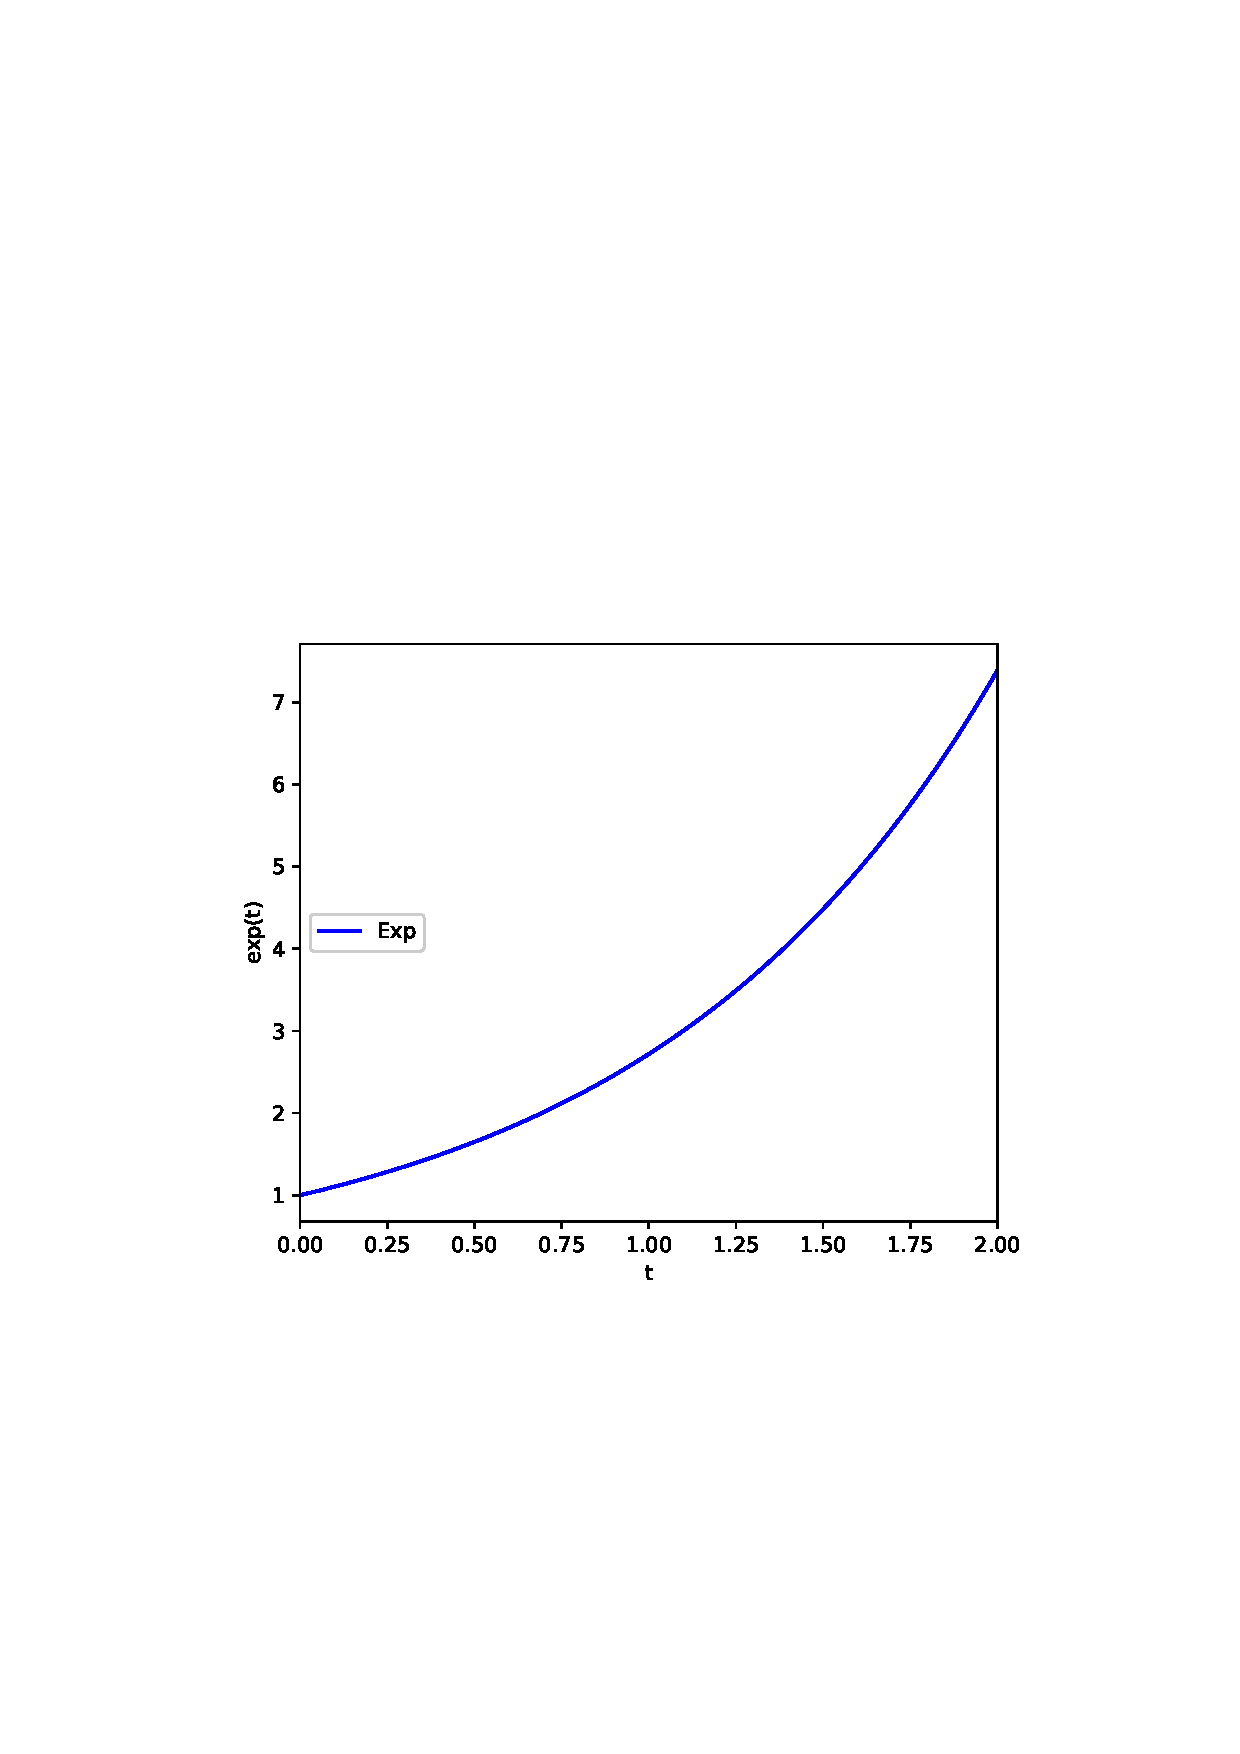
\includegraphics{Fig_test.pdf}
    \caption{Caption}
    \label{fig:my_label}
\end{figure}

\FloatBarrier

Include minimum calculated quality and efficiency of Rankine with and without the reheat cycle. I need to edit the graph to include labels with states.

\section{Conclusions}

This is my conclusion

\appendix

\FloatBarrier % To keep all figures before the references

% produces the bibliography section when processed by BibTeX
\bibliography{Paper_template_bib_file}
\bibliographystyle{aiaa}


\section*{Code Listing}

\lstinputlisting[language=Python]{Great_Code.py}






\end{document}
